% Rafael Sartori M. dos Santos, 186154
\documentclass[brazilian,a4paper,twocolumn]{article}

% Título
\title{MC920 -- Trabalho 4}
\author{Rafael Sartori M. Santos, 186154}
\date{31 de outubro de 2019}

% Configuração do documento
\setlength{\parskip}{3pt}
\usepackage[utf8]{inputenc} % tipo de documento UTF-8
\usepackage{mathtools} % permitir expressões matemáticas
\usepackage{breqn} % equações quebradas em várias linhas automaticamente
\usepackage{babel} % configuração da lingua portuguesa
\usepackage{caption} % para legenda de tabelas e figuras
\usepackage[
    pdfauthor={Rafael Sartori M. Santos},
    pdftitle={Trabalho 4 -- MC920},
    pdfproducer={LaTeX (texlive) com hyperref},
    hidelinks
]{hyperref} % para links externos (href)
\usepackage{cleveref} % para referenciar tabelas e figuras melhor
\usepackage{indentfirst} % indentação de todo primeiro parágrafo
\usepackage{graphicx} % para adicionar imagens
\graphicspath{{../imgs/},{../output/}} % atalho para o caminho das imagens
\usepackage{float} % para fixar posição de imagens
\usepackage{subcaption} % para imagens ficarem lado a lado
% Usamos geometry pois dá mais espaço que fullpage
%\usepackage{geometry} % alterar geometria do papel
%\geometry{a4paper,left=1.7cm,right=1.7cm,top=1cm,bottom=2.0cm} % menor margem
\usepackage{fullpage} % utilizamos uma versão com menos espaçamento nas bordas
\usepackage{verbatim} % pacote para incluir arquivos em verbatim
\usepackage{mdframed} % para enquadrar coisas
\usepackage[bitstream-charter]{mathdesign} % Mudamos a fonte para Charter BT
\usepackage[T1]{fontenc} % Mudamos a fonte para Charter BT

% Início do documento
\begin{document}

\maketitle


\section{Introdução}

    O objetivo do trabalho é a codificação e decodificação de mensagens dentro de imagens e verificar se as novas informações produzem algum artefato visual na imagem. Como exigido pelo enunciado, haverá 2 programas: um para codificação e outro para decodificação.

    Faremos esses programas utilizando Python com as bibliotecas \href{https://opencv.org/}{\emph{OpenCV}}, \href{https://numpy.org/}{\emph{NumPy}}, \href{https://www.pycryptodome.org/}{\emph{pycrypto} (sua implementação atualizada, \emph{pycryptodome})} e padrão.


\section{Metodologia}

    No programa de codificação, precisamos receber uma imagem e um arquivo a ser codificado. Então abrimos essa imagem, alteramos um único \textit{bit} para cada ponto e camada da imagem, escrevendo a mensagem que desejamos, e salvamos a imagem de saída.

    No de decodificação, recebemos a imagem com a mensagem codificada, abrimos e isolamos o \textit{bit} desejado, acumulando num vetor binário que será posteriormente convertido em um arquivo de texto decodificado.

    Com esses passos gerais, começamos preparando a imagem, alterando seu formato em um programa externo.

    \subsection{Preparação da imagem}

        É um requisito trabalhar de forma \textit{lossless} (sem perdas) para manter todas as informações da imagem intactas, garantindo a integridade da mensagem. Isto é, algoritmos de compressão \textit{lossy} podem degradar a imagem e possivelmente causar a corrupção da mensagem.

        Apesar disso, a imagem carregada pelo \emph{OpenCV} não precisa ser de um formato \textit{lossless} pois a biblioteca consegue abrir em um formato e salvar em outro. Há, portanto, apenas uma importância: salvar a imagem sem perdas.

        Para isso, o programa sempre exigirá o formato \texttt{PNG} para a saída, adicionando a extensão ``\texttt{.png}'' caso não esteja mencionado na entrada.

    \subsection{Preparação da mensagem}
    \label{sec:preparacao-mensagem}

        O programa é capaz de encriptar a mensagem de forma segura utilizando uma senha e o algoritmo \texttt{AES}, produzindo um vetor de \textit{bytes}. Caso a senha não seja fornecida, a mensagem é interpretada apenas pelos \textit{bytes} que compõem a \textit{string}.

        Esses \textit{bytes} serão divididos em uma matriz de mesmo tamanho da imagem, contendo apenas um \textit{bit} por posição correspondendo a imagem. Ou seja, dividiremos cada \textit{byte} em 8 \textit{bits} na matriz que possui dimensão igual à da imagem.

        A matriz precisa ser menor ou no máximo de mesmo tamanho à imagem e cada valor precisa ocupar no máximo um \textit{bit}. Caso isso não for verdade, não conseguiremos incluir toda mensagem na imagem sem maiores perdas, pois nos comprometemos pelo enunciado a utilizar apenas um plano de \textit{bits} da imagem. O efeito de qual plano de \textit{bits} devemos escolher para diminuir artefatos visuais será discutido na \cref{sec:efeito-plano-bits} com os resultados.

        Um problema que haverá com esta metodologia é que, como os \textit{bytes} retornados pelo \texttt{AES} não representam um texto em \texttt{ASCII}, não podemos confiar que haverá um caractere terminal \texttt{\textbackslash0}. Devemos, portanto, incluir alguma forma de saber onde a mensagem secreta acaba. Fazemos isso através de um inteiro a ser colocado no preâmbulo: o número de \textit{bytes} da mensagem a ser escrita na imagem.

    \subsection{Colocando a mensagem na imagem}

        Essa etapa é feita através de operações binárias e vetoriais em toda imagem, o que é bastante eficiente e rápido. Começando com a imagem inicial, precisamos remover o trecho da imagem que utilizaremos para a mensagem.

        Fazemos uma máscara $M_m$ que seleciona todas as posições que a mensagem utilizará, pois assim não eliminamos todo o plano de \textit{bits}, apenas as posições que precisamos. Isso dificultará a identificação de uma mensagem dentro da imagem, pois manteremos todo o plano ocupado com informações, e manterá parte da imagem intacta, sobretudo em pequenas mensagens.

        Com a imagem $I$, plano de \textit{bits} $p$ e a máscara $M_m$, zeramos apenas as posições que utilizaremos para a mensagem através da \cref{eq:imagem-sem-plano}, produzindo a imagem ``com vazios'' $I_v$.

        \begin{equation}
        \label{eq:imagem-sem-plano}
            I_v = \texttt{($I$ \&  ($\lnot$($M_m$ << $p$)))}
        \end{equation}


        Juntamos a imagem com espaço para mensagem $I_v$ com a matriz da mensagem $M$ feita na \cref{sec:preparacao-mensagem} através da \cref{eq:imagem-com-mensagem}, resultando na imagem final $I_f$, que agora contém a mensagem no plano de \textit{bits} $p$ especificado.

        \begin{equation}
        \label{eq:imagem-com-mensagem}
            I_f = \texttt{($I_v$ | ($M$ << $p$))}
        \end{equation}

    \subsection{Salvando a imagem final}

        Utilizando \emph{OpenCV}, salvamos a imagem final $I_f$ em formato \texttt{PNG}, que é um formato \textit{lossless}, protegendo a mensagem de degradações.

        Assim, acabamos todas as etapas do codificador. Agora veremos a metodologia para o decodificador, que fará praticamente o trabalho oposto: com a imagem final $I_f$, determinamos a máscara da mensagem $M_m$ e retiramos, utilizando operações binárias novamente, a mensagem $M$. É importante ressaltar que o plano de \textit{bits} $p$ é dado como argumento do programa e não precisa ser determinado pelo decodificador.

    \subsection{Isolando a mensagem}

        Fazemos os mesmos passos para abrir a imagem utilizando \emph{OpenCV}, abrindo a entrada que deve ser dessa vez no formato \texttt{PNG}. Os 4 primeiros \textit{bytes} (divididos entre \textit{bits}, como descrito anteriormente) do plano de \textit{bits} selecionado da mensagem deve conter o tamanho da mensagem a seguir.

        Com o tamanho da mensagem, conseguimos reconstruir a máscara $M_m$ (multiplicamos esse tamanho por 8 -- pois há 8 \textit{bits} dentro de um \textit{byte} -- e decrescemos de 1 em 1 a cada vez que adicionamos, da esquerda para direita, de cima para baixo, um \textit{bit} à máscara vazia exceto pelos 4 primeiros \textit{bytes}).

        Com a máscara pronta, conseguimos isolar a mensagem $M$ através da \cref{eq:isolando-mensagem}.

        \begin{equation}
        \label{eq:isolando-mensagem}
            M = \texttt{($I_f$ \& ($M_m$ << $p$)) >> $p$}
        \end{equation}

        Agora basta isolar \textit{bit} a \textit{bit} a mensagem, formando os \textit{bytes}.

    \subsection{Decodificando a mensagem}

        Com o vetor de \textit{bytes} pronto, se houve a entrada de senha, passamos a mensagem pelo algoritmo de decodificação \texttt{AES}. Com ou sem senha, interpretamos o vetor binário final como uma \textit{string}, obtendo um texto.

        Após exportação do texto para um arquivo, realizamos todas as etapas e a funcionalidade do programa está completa.


\section{Resultados e análise}

    Agora iremos testar a funcionalidade e analisar o efeito da mensagem na imagem em diversos planos de \textit{bits}.

    \subsection{Teste de funcionalidade}

        Para o teste de funcionalidade, codificamos na imagem \texttt{imgs/mel.jpg} a mensagem no arquivo de texto \texttt{input/mensagem.txt} no plano de \textit{bits} 0, produzindo a imagem \texttt{output/mel_coded.png}. Fazemos a decodificação da imagem \texttt{output/mel_coded.png} no plano de \textit{bits} 0 produzindo a mensagem \texttt{output/mensagem_codificada.txt} e notamos que não há qualquer diferença visual entre as duas.

        Utilizamos o parâmetro \texttt{---passphrase}, temos o mesmo resultado. Porém, caso a senha seja incorreta na decodificação, haverá um erro em alguma etapa do algoritmo \texttt{AES}, de conversão para \textit{string} ou, com sorte, o texto ficará ilegível.

        Podemos tentar perceber as diferenças entre a imagem que possui a mensagem e a original na \cref{fig:mel-comparativo}.

        \begin{figure}[h]
            \centering
            \begin{subfigure}{0.23\textwidth}
                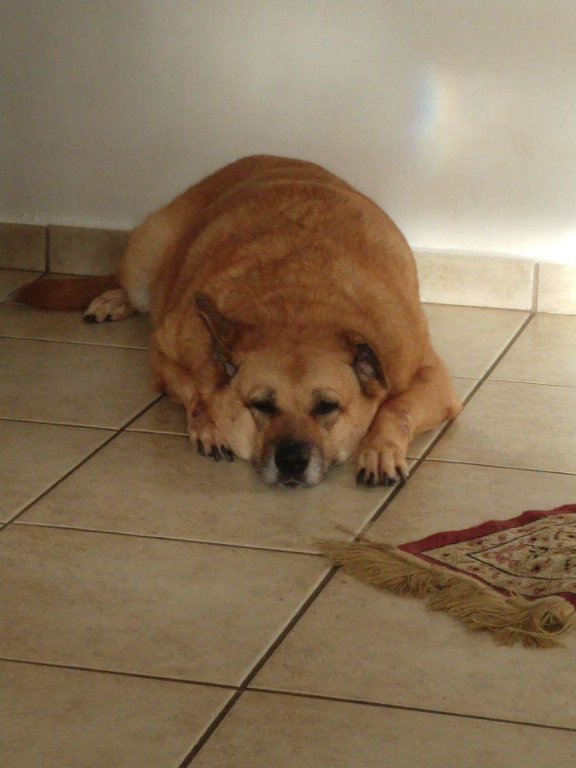
\includegraphics[width=\textwidth,keepaspectratio]{mel}
                \caption{Imagem original}
                \label{fig:mel-original}
            \end{subfigure}
            \hfill
            \begin{subfigure}{0.23\textwidth}
                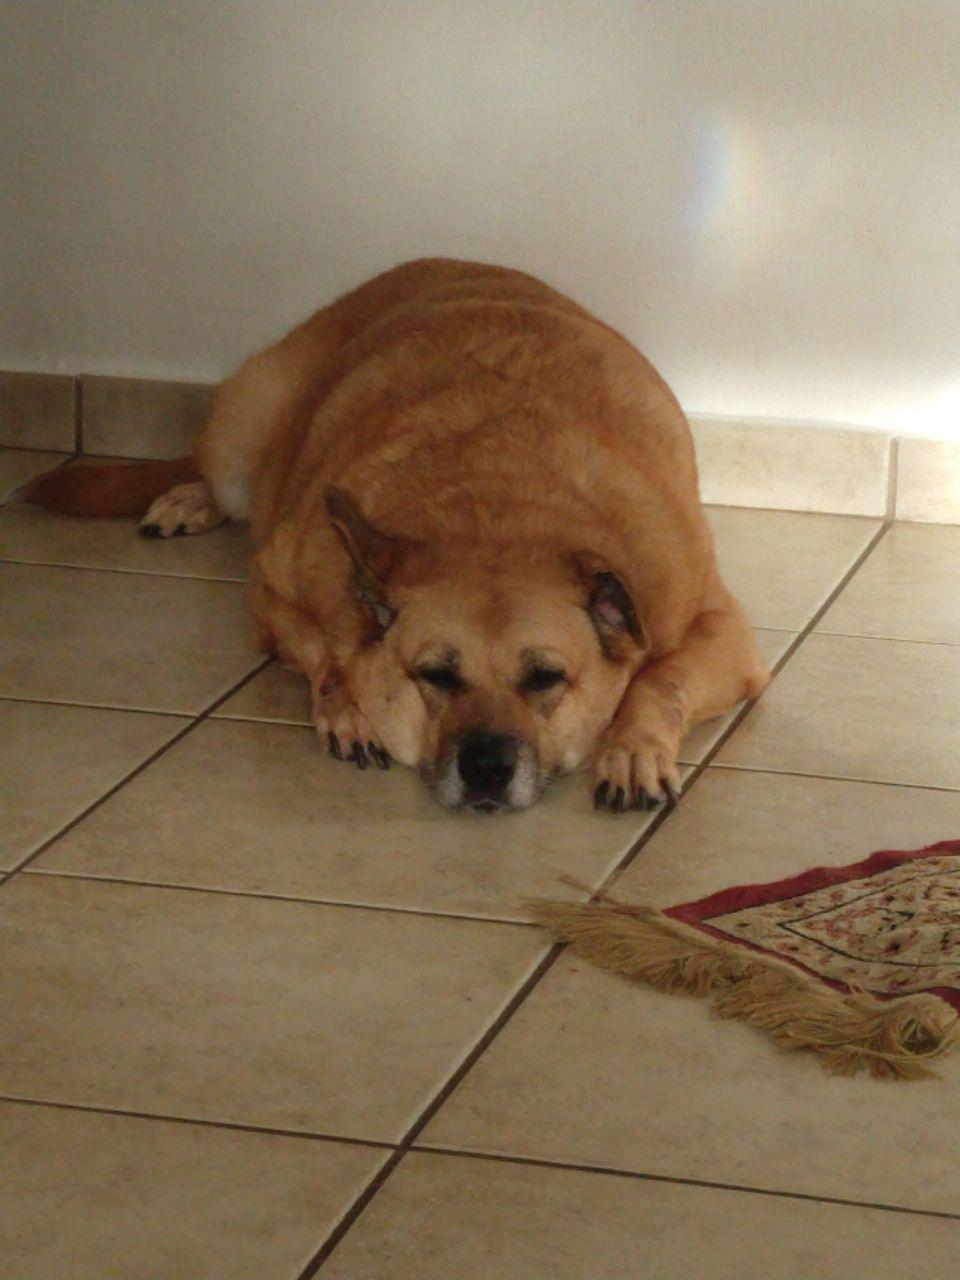
\includegraphics[width=\textwidth,keepaspectratio]{mel_coded}
                \caption{Imagem codificada}
                \label{fig:mel-coded}
            \end{subfigure}

            \caption{Comparativo entre a imagem original e a com mensagem codificada.}
            \label{fig:mel-comparativo}
        \end{figure}

    \subsection{Análise de espaço}
    \label{sec:espaco-utilizado}

        A mensagem utiliza espaço que antes era destinado à informações da imagem, inevitavelmente produzindo artefatos e degradando a imagem, por mais que pequenas. A capacidade de armazenar dados dentro de uma imagem comum atual é bastante grande visto que os \textit{bits} menos significativos produzem pouca interferência visual e a dimensão é grande mesmo em celulares mais modestos.

        Em uma imagem tradicional que utilizamos no dia a dia, teremos geralmente 3 camadas de cores com profundidade de 8 \textit{bits}. Como utilizamos apenas um plano, apenas 1 desses 8 \textit{bits} poderão ser utilizados. Considerando a imagem com largura $w$ e altura $h$, teremos $ 3 \cdot w \cdot h / 8 $ \textit{bits} para escrever a mensagem.

        No entanto, podemos utilizar planos independentes entre si. Ou seja, se quisermos, podemos utilizar todos os 8 planos disponíveis, efetivamente destruindo a imagem original, utilizando todos os pontos somente para a mensagem. Exemplifico isso na \cref{fig:mel-coded-todos}, onde todos os planos foram ocupados com a mesma mensagem (que ocupa apenas um trecho da imagem). Apesar de visualmente terrível, devido a compressão do formato \texttt{PNG}, economizamos espaço comparado ao arquivo de texto padrão do sistema.

        \begin{figure}[h]
            \centering
            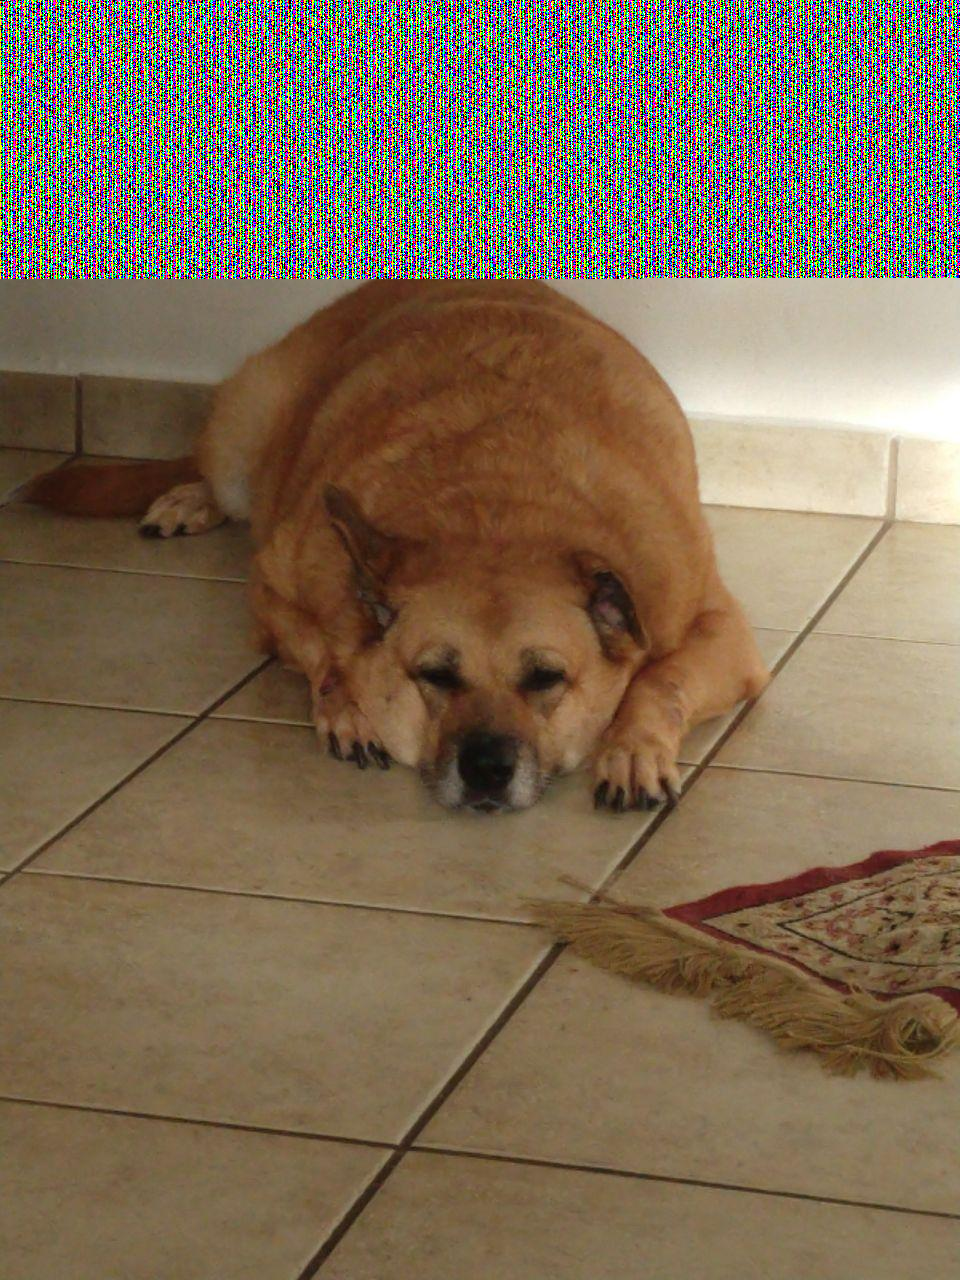
\includegraphics[width=0.4\textwidth,keepaspectratio]{mel_coded_all}
            \caption{Imagem codificada em todos os planos.}
            \label{fig:mel-coded-todos}
        \end{figure}

    \subsection{Análise dos planos de \textit{bits}}
    \label{sec:efeito-plano-bits}

        Podemos verificar na \cref{fig:comparativo-planos} o efeito visual negativo causado pela mensagem em planos de \textit{bits} mais significativos da imagem, alterando cada vez mais significativamente as cores de fato.

        Confirmamos ainda o trecho da imagem que é utilizado para a mensagem, comentado na \cref{sec:espaco-utilizado}, já que o programa nos informou que utilizamos cerca de $20\%$ da capacidade total do plano da imagem e visualmente parece correto: cerca de um quinto da imagem é visualmente afetada na \cref{fig:comparativo-plano-7}.

        \begin{figure*}
            \centering
            \begin{subfigure}{0.18\textwidth}
                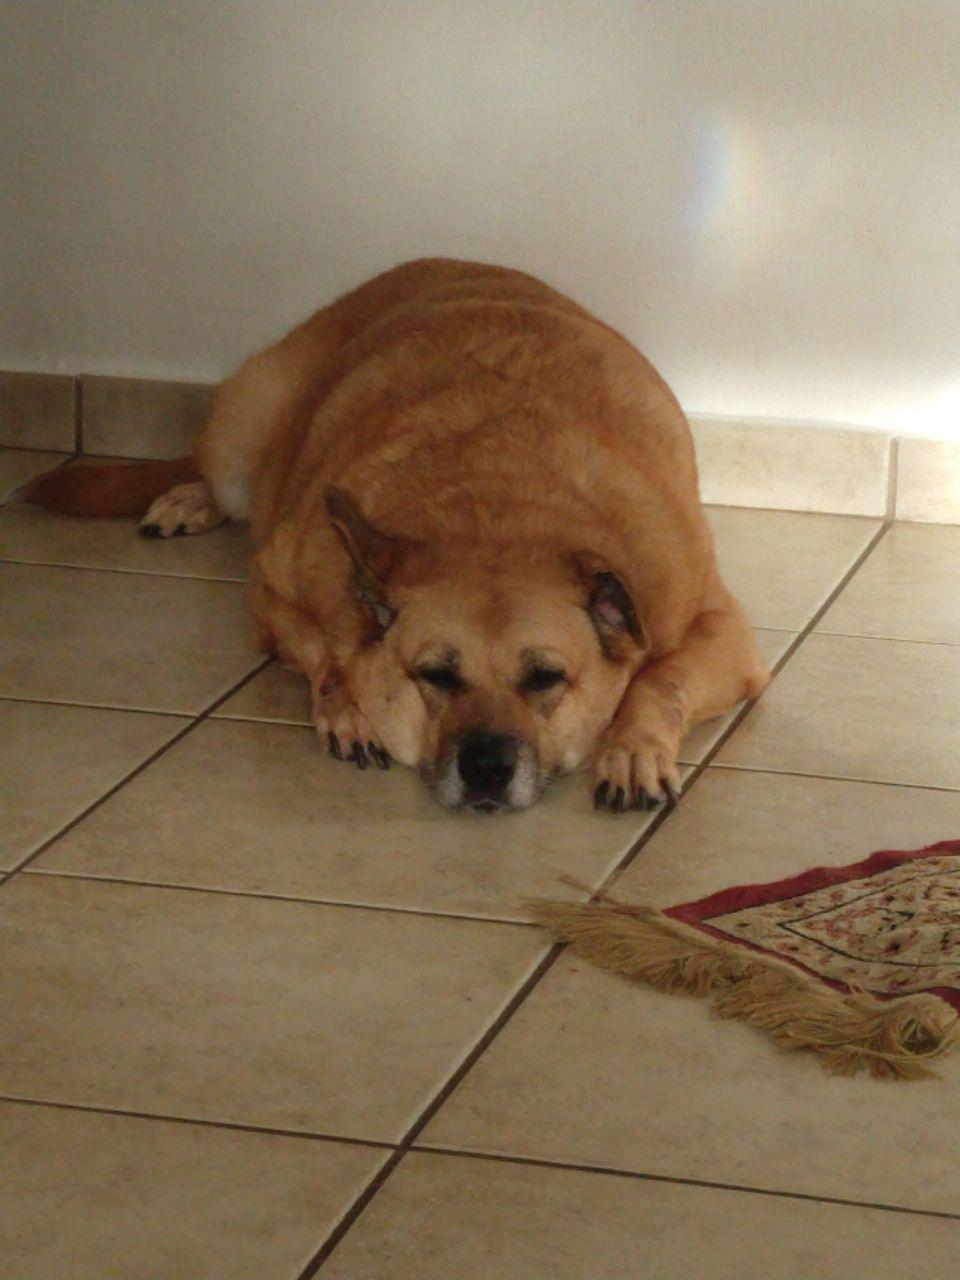
\includegraphics[width=\textwidth,keepaspectratio]{mel_coded}
                \caption{No plano $0$}
            \end{subfigure}
            \hfill
            \begin{subfigure}{0.18\textwidth}
                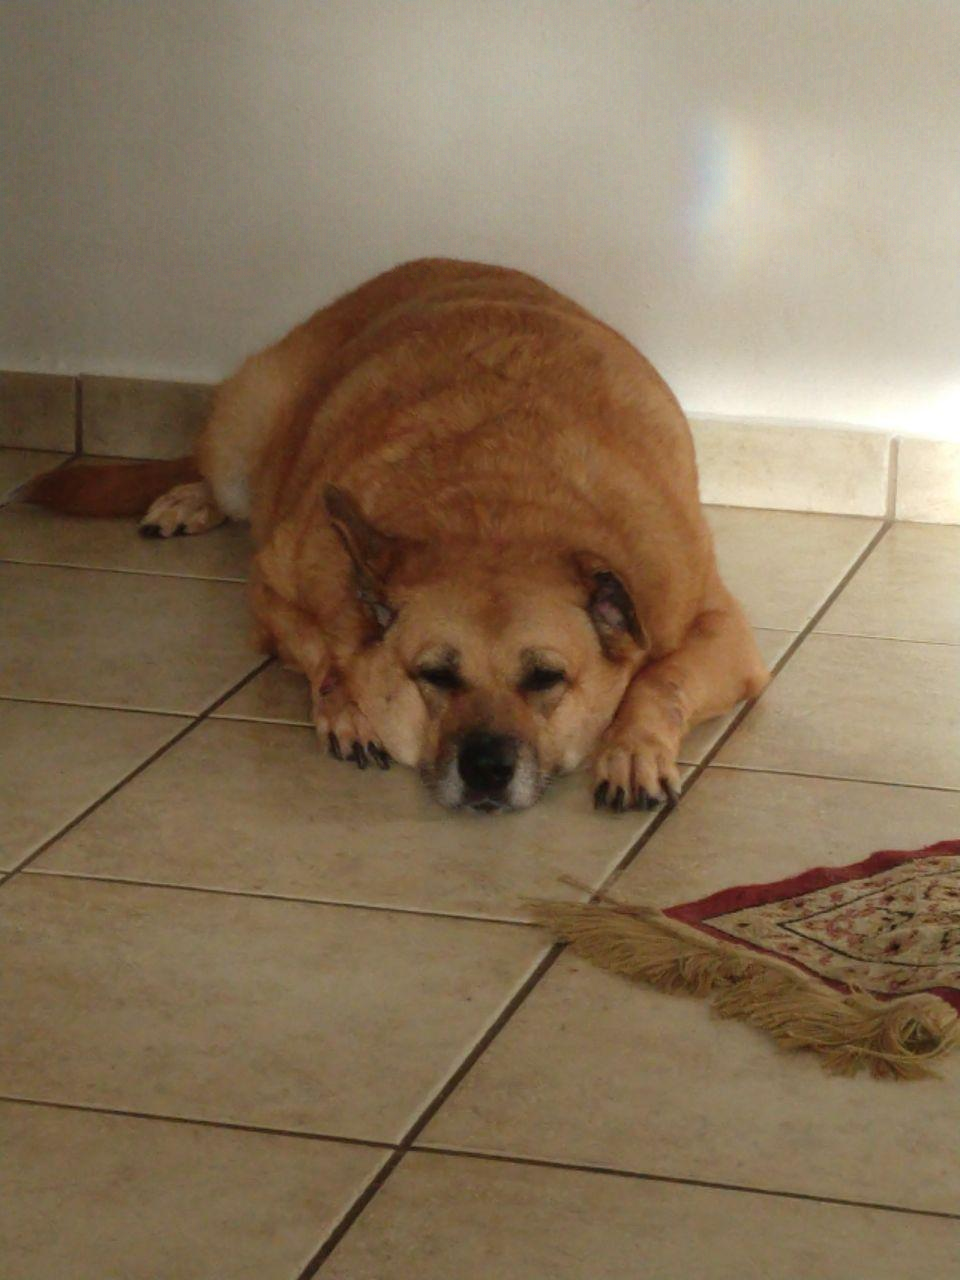
\includegraphics[width=\textwidth,keepaspectratio]{mel_coded_1}
                \caption{No plano $1$}
            \end{subfigure}
            \hfill
            \begin{subfigure}{0.18\textwidth}
                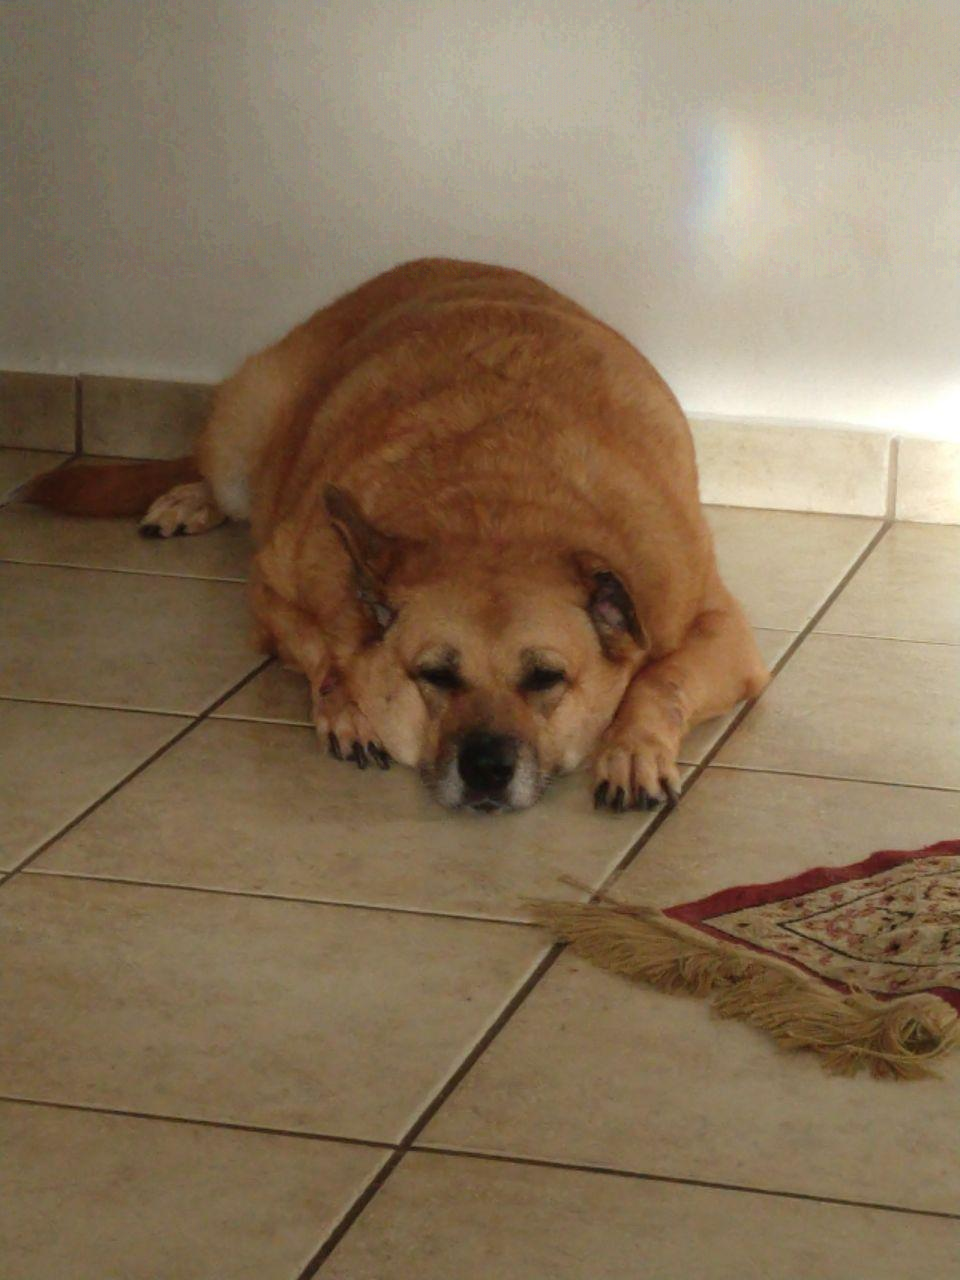
\includegraphics[width=\textwidth,keepaspectratio]{mel_coded_2}
                \caption{No plano $2$}
            \end{subfigure}
            \hfill
            \begin{subfigure}{0.18\textwidth}
                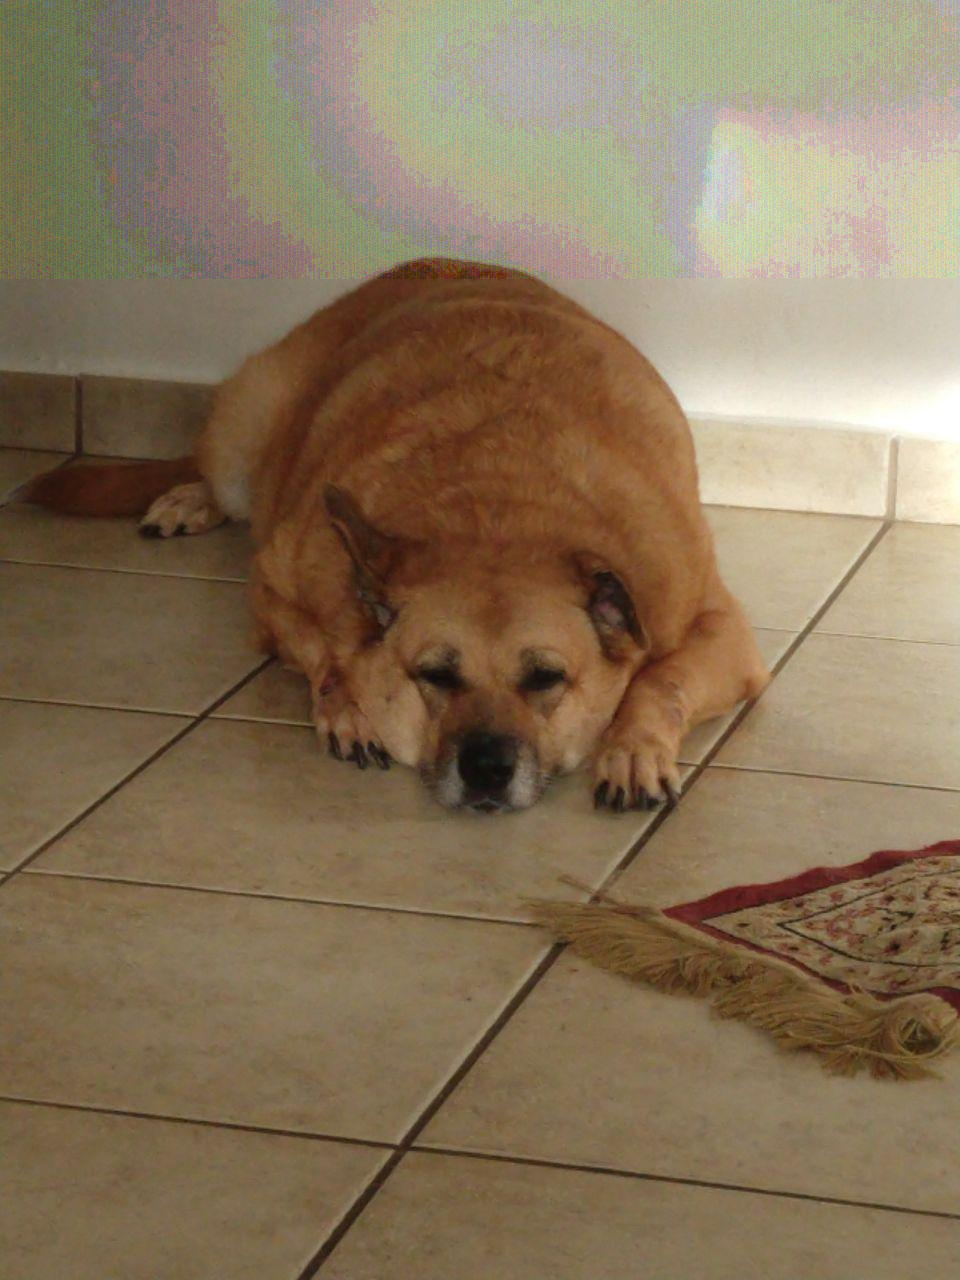
\includegraphics[width=\textwidth,keepaspectratio]{mel_coded_4}
                \caption{No plano $4$}
            \end{subfigure}
            \hfill
            \begin{subfigure}{0.18\textwidth}
                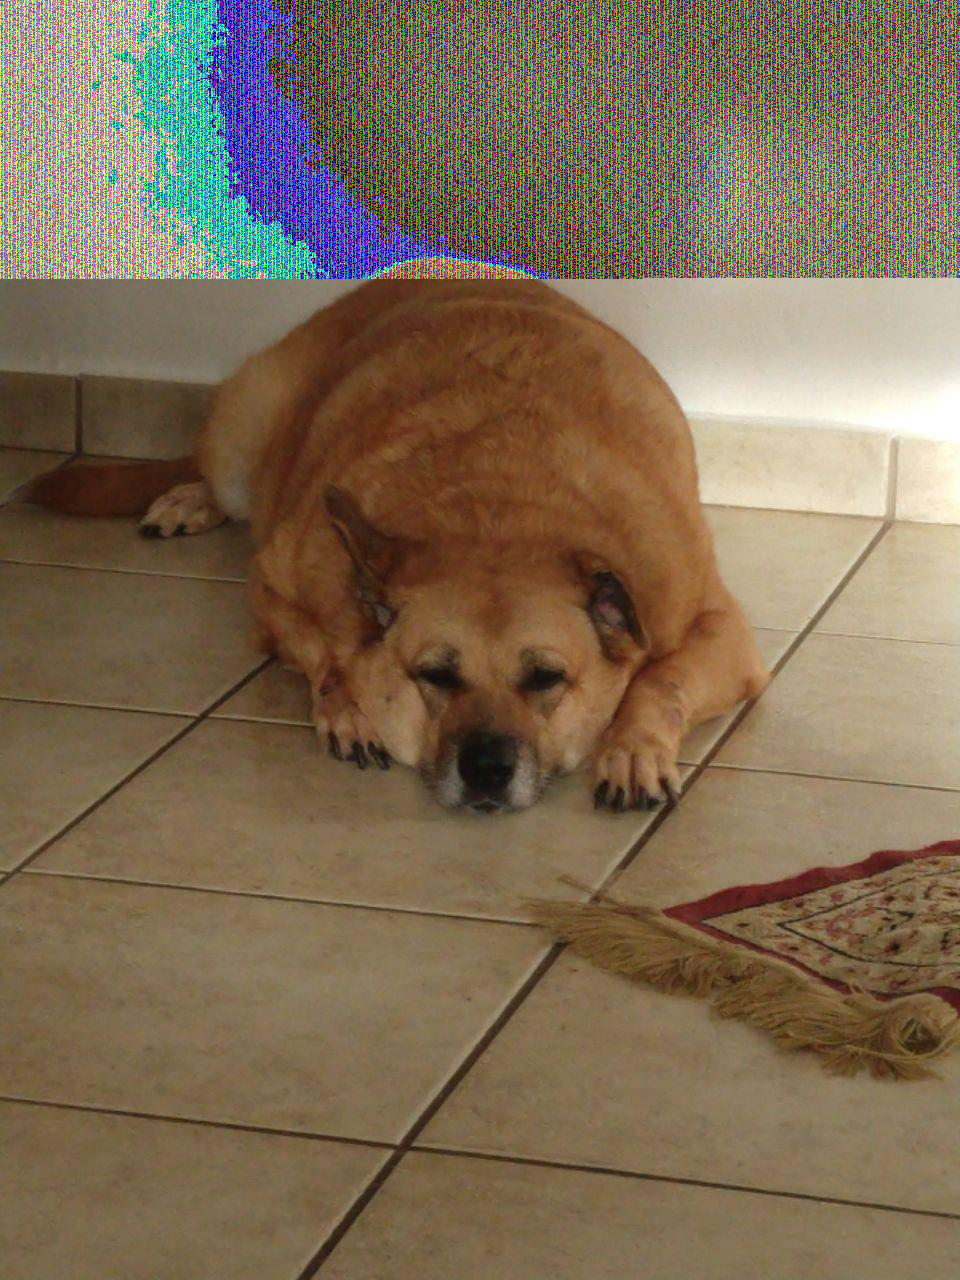
\includegraphics[width=\textwidth,keepaspectratio]{mel_coded_7}
                \caption{No plano $7$}
                \label{fig:comparativo-plano-7}
            \end{subfigure}

            \caption{Comparativo entre planos de \textit{bits} utilizados para codificar a mensagem.}
            \label{fig:comparativo-planos}
        \end{figure*}

\end{document}
